\documentclass[9.5pt,journal,letterpaper,compsoc]{IEEEtran}
\usepackage[cmex10]{amsmath}
\usepackage{graphicx, latexsym,amssymb}

%\setlength{\evensidemargin}{0in}
%\setlength{\oddsidemargin}{0in}
%\setlength{\textwidth}{6.6in}
%\setlength{\columnwidth}{86mm}
%\setlength{\textheight}{8.5in}
%\setlength{\topmargin}{0in}
%\setlength{\headheight}{.4in}
%\setlength{\headsep}{.1in}

\newtheorem{theorem}{\bf Theorem}[section]
\newtheorem{definition}{\bf Definition}[section]
%\newtheorem{proposition}{Proposition}[section]
\newtheorem{lemma}{\bf Lemma}[section]
%\newtheorem{corollary}{Corollary}[section]

\begin{document}

\title{From Gene Trees to Species Trees II: \\
   Species Tree Inference by Minimizing  Deep Coalescence Events}
\author{Louxin~Zhang
\IEEEcompsocitemizethanks{\IEEEcompsocthanksitem Louxin Zhang is with
the Department of Mathematics, National University of Singapore,
10 Lower Kent Ridge Road, Singapore 119076. \protect\\
 Email: matzlx@nus.edu.sg
}
\thanks{}
}


 %The paper headers
\markboth{IEEE/ACM TCBB}{Zhang: Species Tree Inference By Minimizing Deep Coalescence Events}



\IEEEcompsoctitleabstractindextext{ %
\begin{abstract}
 When gene copies are sampled from various species, the resulting gene tree
might disagree with the containing species tree.
The primary causes of gene tree and species tree discord include
 incomplete lineage sorting, horizontal gene transfer, and gene
duplication and loss. Each of these events yields a different
parsimony criterion for inferring the (containing) species tree from
gene trees.  With incomplete lineage sorting, species tree inference
is to find the tree minimizing extra gene lineages that had to
coexist along species lineages; with gene duplication, it becomes to
find the tree minimizing gene duplications and/or losses. In this
paper, we present the following results:

(i)  The deep coalescence cost is equal to the number of
 gene losses minus two times the gene duplication cost in
the reconciliation  of  a uniquely leaf labeled gene tree and a species
tree. The deep coalescence cost can be computed in linear time
for any arbitrary gene tree and species tree.

(ii)  The deep coalescence cost is always no less than the gene
duplication cost in the reconciliation of an arbitrary gene tree and
a species tree.

(iii) Species tree inference by minimizing deep coalescence events
is NP-hard.
\end{abstract}

\begin{IEEEkeywords}
 Gene tree and species tree reconciliation, deep coalescence,
gene duplication and loss, the Parsimony principle, NP-hardness.
\end{IEEEkeywords}
}

\maketitle

\IEEEdisplaynotcompsoctitleabstractindextext
\IEEEpeerreviewmaketitle

\section{Introduction}
\IEEEPARstart{G}{ene} trees are fundamental to molecular
systematics. Traditionally, a gene tree is reconstructed from  DNA
sequence variation at individual genetic loci in a group of species
and is taken as the phylogenetic tree of the species due to
sequencing technology limitations. However,  when gene copies are
sampled from various species, the resulting gene tree might disagree
with the species tree.  As such, the relationship between gene trees
and species trees has been the focus of many studies (see for
example \cite{Doyle_SysBot_92, Goodman_SysZool_79,
Maddison_SysBiol_97, Page_SysBiol_94, PN88, T89, Wu91}). It has long
been recognized that gene trees can be used to estimate species
divergence time, ancestral population sizes and
 even the containing species tree although they
 may not accurately
reflect the species tree \cite{Edwards_Evolution_00,
Hey_Genetics_04, Maddison_SysBiol_06}.

The discord of gene trees and the containing species tree can arise
from horizontal gene transfer, incomplete lineage sorting, and gene
duplication and loss. The importance of these causes depends on the
considered  genes and species. Hence, inferring the species tree
from gene trees has been investigated under various parsimony
criteria. With incomplete lineage sorting (also called deep
coalescence), the problem is to find the tree minimizing
 extra gene lineages that had to coexist along species
lineages \cite{Maddison_SysBiol_97}; with gene duplication, it becomes
to find the tree minimizing gene duplications and/or losses
\cite{Goodman_SysZool_79, Page_SysBiol_94, Guigo_MPE_96,Ronquist_ZoolScr_97}.


Inferring the species tree from a set of gene trees has often been
studied under the gene duplication cost \cite{Bansal_TCBB_08,
Chauve_JCB_08, Chen_JCB_00, Durand_JCB_06, Eulenstein_JCB_98,
Hallett_Recomb00, Hadas_JCB_09, Luo_TCBB_10, Roth_JExpZool_07,Zh97}
until very recently. In a seminal work \cite{Maddison_SysBiol_97},
Maddison addressed incomplete lineage sorting in the framework of
coalescence theory. Coalescence theory is an active branch of
population genetics concerned with tracing the genealogical history
of a present-day gene copy. For a gene sampled from two individuals,
one may ask: How deep in time do these two lineages coalesce? Hence,
the depth of this coalescence is  a measure of the relationship
between two sampled gene copies. The more deep in time coalescence
occurs, the more distantly related they are.  Maddison proposed to
use the total number of ``extra" gene lineages that fail to coalesce
on a species tree
 to measure the inconsistence of a gene tree and the species tree,
called the {\it deep coalescence cost}. For the gene tree and
species tree shown in Fig.~\ref{DCExample},  there are three gene
lineages
 on a branch and two gene lineages on  another branch
that fail to coalesce, giving the deep coalescence cost of 3.
 Since coalescence
theory provides the probability that a gene tree would exist in a
species tree, it allows the inference problem to be studied in an
explicitly statistical framework \cite{Degan_Evol_05,
Rosenberg_TheorPopBiol_2002}. This seems to give the deep
coalescence model an advantage over the other models.


This paper is a sequel of \cite{Ma_SIAMComput_01} that studies the
complexity and algorithmic issues of inferring the species tree from
a set of gene trees with the gene duplication/loss cost in the
reconciliation of a gene tree and the containing species tree.
Here, we present an equation of the deep coalescence cost, the
duplication cost, and the number of gene losses. We also show that
the deep coalescence cost is  no less than  the gene duplication
cost. Although deep coalescence and gene duplication are two
different mechanisms responsible for the discord of gene trees and
species trees, this relationship suggests that the deep coalescence
cost and the duplication cost are closely related to each other as a
similarity measure of trees. We further show that inferring species
tree from gene trees by minimizing the deep coalescence cost is also NP-hard.



\begin{figure}[bth!]
\begin{center}
\includegraphics[width=0.7\columnwidth]{Figure1.eps}
\end{center}
\caption{(i) A gene tree. (ii) A species tree. (iii)
  The reconciliation of  the gene tree in (i) and the species tree in (ii) has
deep coalescence cost 3.
\label{DCExample}
}
\end{figure}

\section{Basic Definitions and Notations}

In this section, we shall introduce basic definitions and notations on
gene duplication, gene loss and deep coalescence that are used in
 the rest of the paper.

\subsection{Species Trees and Gene Trees}

For a set of $n$ taxa, their evolutionary history is modeled as a rooted, full
binary tree with $n$ leaves in which leaves are uniquely labeled with taxa,
 representing the labeling taxa,
and internal nodes are unlabeled.   Here, the `fullness' means that
each internal node has exactly two children. Such a tree is called a
{\it species tree}. In a species tree, each unlabeled internal node
is considered as a {\it taxon family} which include as its members
the subordinate species represented by the leaves below it. Thus,
the evolutionary relation ``$m$ is a descendant of $n$" is expressed
using the set-theoretic notation as ``$m\subsetneq n$".
  We also call an internal node  an {\it ancestor} of the species below it.

The model for gene evolutionary relationship is also a rooted, full
binary tree with leaves representing genes, called a {\it gene
tree}. Usually, a gene tree is reconstructed from a collection of
gene  family members sampled from the considered species. We label
the gene copies by the species from which they are sampled. In a
gene tree, leaf labels may not be unique as two or more  gene copies
might  be sampled in a species. An internal node $g$ corresponds to
a multiset of leaf labels.

Finally, for a species or  gene tree $T$, we use $L(T)$ to denote
the set of leaf labels of it.  We write $t\in T$ to denote that $t$
is an internal node of $T$. For any $t\in T$, $a(t)$ and $b(t)$ are
used to denote its two children.

\subsection{Gene Duplication}

Let $G$ be a gene tree and $S$ a species tree such that
$L(G)\subseteq L(S)$. For any nodes  $s', s''$ in $S$, the {\it
least common ancestor} of $s'$ and $s''$ is defined to be the
internal node $s\in S$ satisfying that $s', s''\subseteq s$, but the
children of $s$ do not have this containment  property, which is
denoted by $\mbox{lca}(s', s'')$.  To reconcile  $G$ and
 $S$, each node $g$ of $G$ is mapped
to a unique node $M(g)$ in $S$ as
\begin{eqnarray*}
 M(g)=\left\{ \begin{array}{ll}
              \mbox{the leaf of $S$ with the same label},
& \mbox{$g$ is a leaf,}\\
            \mbox{lca}\left(M(a(g)), M(b(g))\right), & \mbox{otherwise}.
          \end{array}
        \right.
\end{eqnarray*}
%
This mapping $M$ was first considered in \cite{Goodman_SysZool_79}
and then formulated in \cite{Page_SysBiol_94}. We call $M$ the
$\mbox{lca}$ mapping or reconciliation of $G$ with $S$. Obviously,
if $g'\subseteq g$, $M(g') \subseteq M(g)$.

\begin{definition}
 Let $g$ be an internal node of $G$. If
 $M(c(g))=M(g)$ for some child $c(g)$ of $g$, then
we say that  a duplication occurs at $M(g)$ (or more exactly
in the lineage entering $M(g)$) in $S$.
\end{definition}

The total number of duplications arising in the lca reconciliation of
 $G$ in  $S$ is proposed to measure the discord
of the gene tree and species tree  and is called the
{\it duplication cost}. We use $c_{dup}(G, S)$ to denote the duplication cost
for $G$ and $S$. Note that the duplication cost is not symmetric.

\subsection{Gene Loss}

A subset $A$ of nodes of a species tree $S$ is
 incomparable if, for any $x, y\in A$, one is not an ancestor of the other.
 For an incomparable subset $A$ in $S$, the restriction of $S$ on $A$ is the smallest
subtree of $S$ containing $A$ as its leaf set, denoted by $R_S(A)$.
It is easy to see that the root of $R_S(A)$ is the least common
ancestor of the nodes from $A$. The homomorphic subtree $S|_A$ of
$S$ induced by $A$ is a tree obtained from $R_S(A)$ by contracting
all degree-2 nodes except for the root of $R_S(A)$.

Let $G$ be a gene tree such that  $L(G)\subseteq L(S)$.
 $S|_{L(G)}$ is well defined.
To reconcile $G$ and $S$ in this general case, we consider the lca
mapping $M$ from $G$ to $S|_{L(G)}$. For any two nodes  $s$ and $s'$
of $S|_{L(G)}$ such that $s\subsetneq s'$,
 we define
$$
 d(s, s')=|\{ h\in S|_{L(G)}\;:\; s \subsetneq h \subsetneq s'\}|.
$$
That is, $d(s, s')$ is the number of nodes on the path from $s'$ to
$s$ excluding $s$ and $s'$.

Recall that $a(g)$ and $b(g)$ denote the children of $g$. The number
of losses $l_g$ associated with $g$ is defined as
\begin{eqnarray*}
l_g=\left\{ \begin{array}{ll}
  0, &\hspace{-1em}  \mbox{ if } M(g)=M(a(g))=M(b(g)),\\
f(a(g)) +1, & \hspace{-1em} \mbox{ if }  M(a(g))\subsetneq M(g)= M(b(g)),\\
\sum_{h=a(g),b(g)}f(h), & \hspace{-1em} \mbox{ if }
M(a(g)), M(b(g))\subsetneq M(g),
\end{array}
\right.
\end{eqnarray*}
where, for a non-root node $x$ in $G$, $f(x)=d\left(M(x),
M\left(p(x)\right)\right)$ in which $p(x)$
 denotes the parent of $x$.
%
 This definition of $l_g$ is a generalization of  the loss cost given
in \cite{Guigo_MPE_96}. When $L(G)=L(S)$, our definition  is then
identical to the one given in \cite{Guigo_MPE_96}.

The {\it gene loss cost} of the reconciliation of $G$ in $S$ is
defined as the total number of losses $\sum_{g\in G} l_g$. We denote
this gene loss cost for $G$ and $S$  by $c_{loss}(G, S)$.

\subsection{Deep Coalescence}

Let $G$ be a gene tree and $S$ a species tree such that $L(G)=L(S)$.
Under the lca reconciliation $M: G\rightarrow S$, if a branch $e$ of
$S$ is on the $k$ paths from $M(g_i)$ to $M(c(g_i))$, $g_i\in G$
($1\leq i\leq k$),  then we say that there are $k-1$ `extra'
lineages failing to coalesce on  $e$. The {\it deep
coalescence}~(DC) {\it cost} is defined as the total number of the
`extra' lineages on all branches of $S$ in the reconciliation $M$ of
$G$ with $S$ (see \cite{Maddison_SysBiol_97}), which is denoted by
$c_{dc}(G, S)$. Note that the concept of deep coalescence is
meaningful only if $S$ has 2 or more leaves. We assume this fact
throughout the paper.

In general, if $L(G)\subseteq L(S)$, the deep coalescence cost
$c_{dc}(G, S)$ is defined as $c_{dc}(G, S|_{L(G)})$, where
$S|_{L(G)}$ is the homomorphic subtree of $S$ induced by $L(G)$.
Such a generalization will be used in the study of inferring the
species tree from a set of gene trees


\section{An Equation of the Duplication, Loss  and  DC Costs}

 We have seen that  deep coalescences, gene losses and duplications
are inferred through gene tree and species tree reconciliation.
In fact,  the number of these events
 are indeed closely related through a simple equation.


\begin{definition}
 Let $G$ be a gene tree and $S$ a species tree such that $L(G)\subseteq L(S)$.
Under the lca  reconciliation ${M}: G\rightarrow S$,
an internal node  $g\in G$ is of
 \begin{itemize}
  \item  type-1 if $M(g') \subsetneq M(g)$ for every child $g'$ of $g$;
  \item  type-2 if there exists a unique child $g'$ such that $M(g') =
M(g)$;
  \item type-3  if $M(g')=M(g)$ for  every child $g'$ of $g$.
 \end{itemize}
\end{definition}

 Note that type-2 or type-3 internal nodes correspond one-to-one with duplication events.

\begin{theorem}
\label{thm31}
Let $G$ be a uniquely leaf-labeled gene tree and $S$ a species tree such
that $L(G)=L(S)$. Then,
  $$ c_{dc}(G, S) = c_{loss}(G, S) - 2c_{dup}(G, S).$$
\end{theorem}
\begin{proof}
Let $G$ and $S$ have $n$ leaves.
Assume that there are $k_1$ type-1 internal nodes
 $$ g_{11}, g_{12}, \ldots,  g_{1k_1},$$
$k_2$ type-2 internal nodes
 $$ g_{21}, g_{22}, \ldots, g_{2k_2}, $$
 and $k_3$ type-3  internal nodes
$$ g_{31}, g_{32}, \ldots, g_{3k_3}$$
in $G$ under the lca  reconciliation $M: G\rightarrow S$, respectively.
Since $G$ is a full binary tree with $n$ leaves, $G$
has   $n-1$ internal nodes and hence
\begin{eqnarray}
\label{node_partition}
 k_1+k_2+k_3 = n-1.
\end{eqnarray}
Additionally,  type-2 and type-3 nodes correspond one-to-one with
duplication events,
\begin{eqnarray}
\label{dup_cost}
  c_{dup}(G, S)= k_2+k_3.
\end{eqnarray}
For simplicity, we assume that
 $g'$ and $g''$ are the children of $g$ for each type-1 internal node $g$;
we also assume  that $a(g)$ is the
unique child such that $M\left(a(g)\right)\subsetneq M(g)$
for each type-2 node $g$.
Since we use  $d\left(M(h), M(g)\right)$ to denote the number of
nodes on the path from $M(g)$ to $M(h)$ for a node $g$ and its child $h$,
the number of lineages contained in the path is
$d\left(M(h), M(g)\right)+1$.  Therefore,
by Eqn.~(\ref{node_partition}) and~(\ref{dup_cost}) and  the fact that $|E(S)|=2n-2$,
\begin{eqnarray*}
  c_{dc}(G, S)& =& \sum ^{k_1} _{j=1}  \left\{ \left[d\left(M(g'_{1j}),
M(g_{1j})\right)+1\right]\right. \\
 & &\;\;\;\;\; \left. + \left[d\left(M(g''_{1j}), M(g_{1j})\right)+1\right]\right\}\\
 & & + \sum ^{k_2} _{j=1} \left[d\left(M(a(g_{2j})), M(g_{2j})\right)+1\right] -|E(S)|\\
  & = & c_{loss}(G, S) + 2k_1 - (2n-2)\\
  & = & c_{loss}(G, S) -2(k_2+k_3) \\
  &=  &  c_{loss} (G, S) - 2c_{dup}(G, S).
\end{eqnarray*}
This concludes the proof.
\end{proof}
\vspace{1em}



\noindent {\bf Remarks}. (i) Following the proof of the equation in
the above theorem, one can easily see that for an arbitrary gene
tree $G$ in which there may be two or more gene copies from a
species and a species tree $S$ such that $L(G)\subseteq L(S)$,

%\begin{center}
\begin{eqnarray}
\hspace{-1em} && c_{dc}(G, S) \nonumber \\
\hspace{-1em} &=& c_{loss}(G, S) - 2c_{dup}(G, S) +
\left(|G|-|R_S(L(G))|\right) \label{eqn_general}
\end{eqnarray}
%\end{center}
 where $|T|$ denotes the number of
the nodes of $T$ for $T=G, R_{S}(L(G))$.  Note that when $L(G)\neq
L(S)$, $G$ is mapped onto $R_{S}(L(G))$, which is the restriction of
$S$ on the set of leaves whose labels are in $L(G)$
and may not be a fully binary tree.

(ii) With the presence of multiple gene copies, the last term in the
right-hand side of  Eqn~(\ref{eqn_general}) is the size difference
of the gene tree and species tree. Since ancient gene duplication
produces more gene copies than recent gene duplication, the deep
coalescence cost penalizes ancient gene duplication more than recent
one if gene loss is rare. This fact suggests that the deep
coalescence cost might be more suitable for inferring recent
duplication events than the gene duplication cost.

(iii) Since the number of gene  duplications and losses can be
calculated in linear time \cite{Zh97, Ma_SIAMComput_01}, the first
remark implies that the deep coalescence cost can also be computed
in linear time.
% \vspace{1em}


 By Theorem~\ref{thm31}, $c_{dc}(G, S)\leq c_{loss}(G, S)$ for a species tree $S$
and a uniquely leaf labeled gene tree $G$. Now we show that the DC
cost is also  bounded below by the duplication cost for any
arbitrary gene trees.

\begin{figure}
\begin{center}
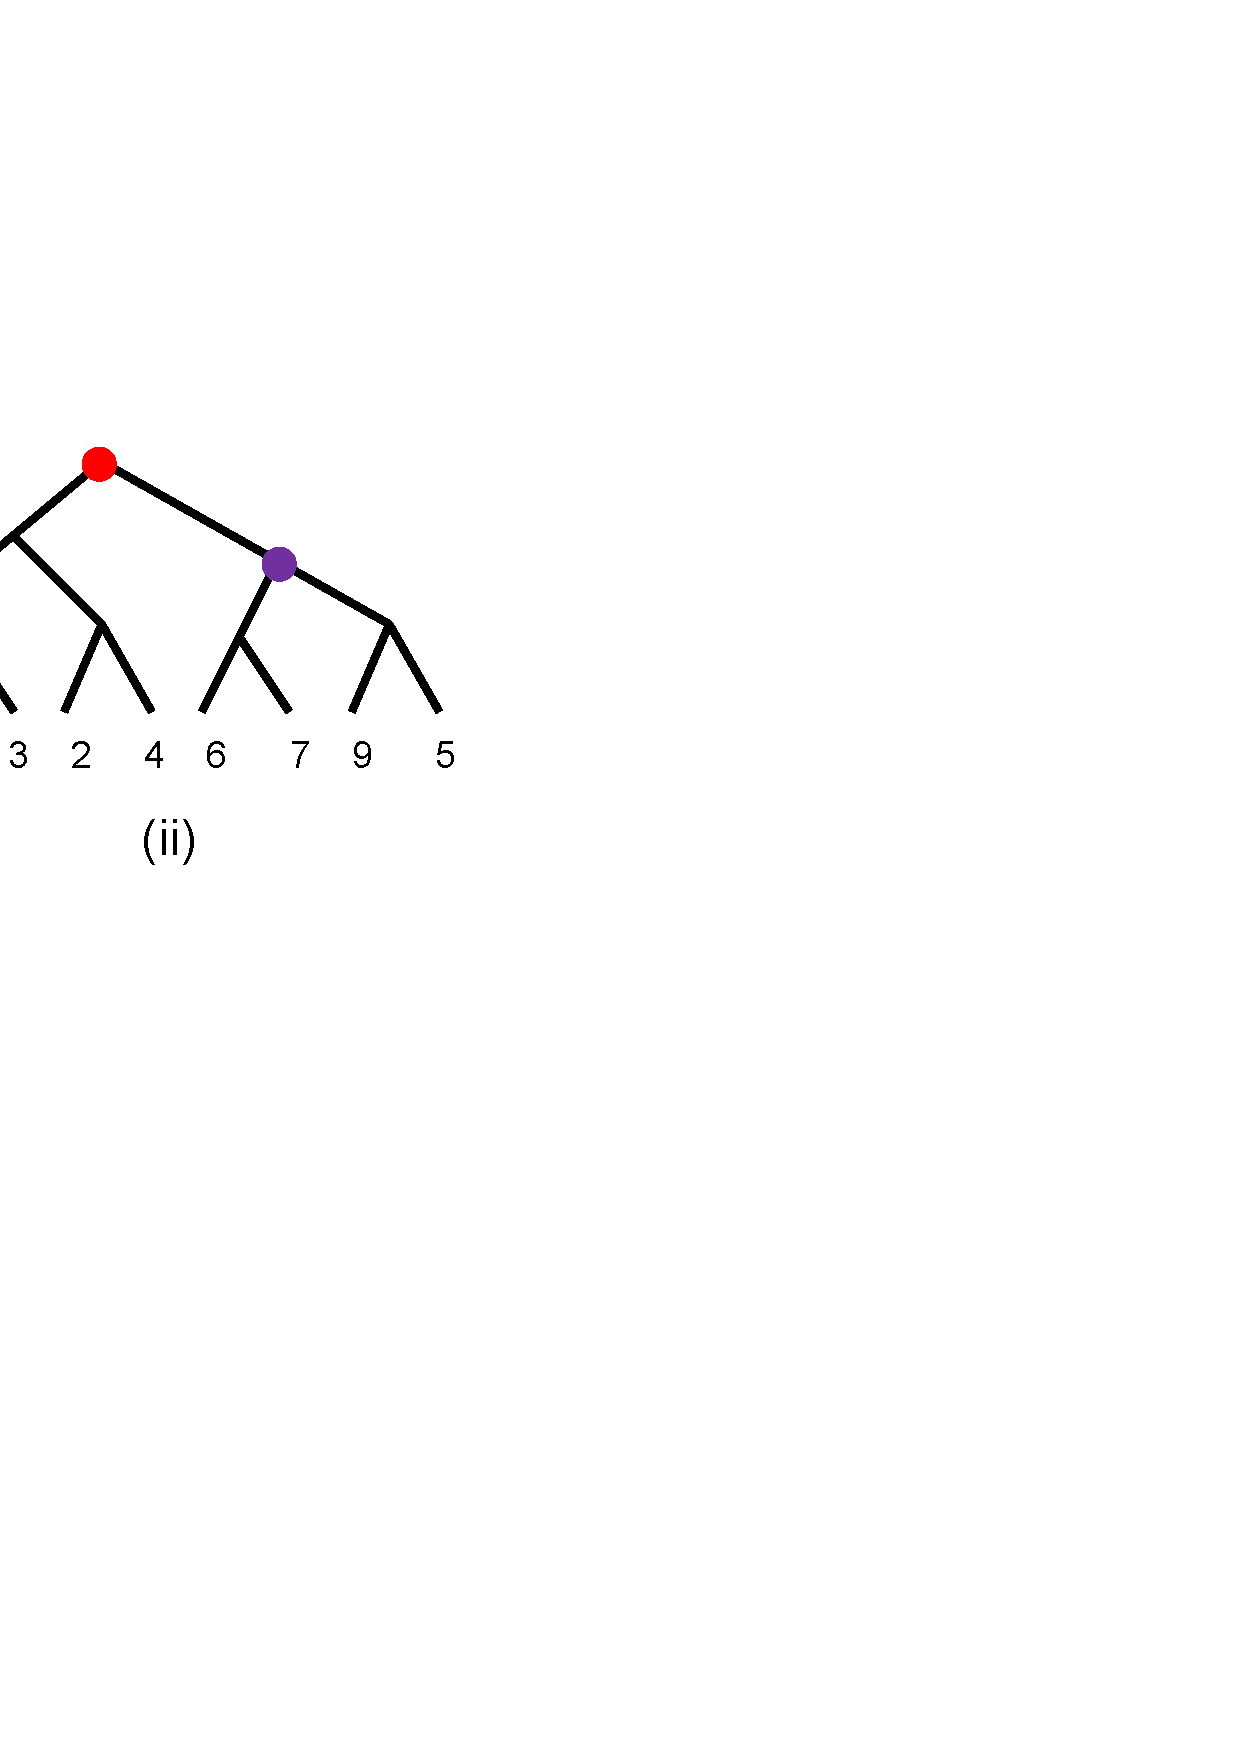
\includegraphics[width=0.9\columnwidth]{Figure2}
\end{center}
\caption{(i) A gene tree. (ii) A species tree. In the lca  reconciliation $M$
  of the gene tree with the species tree,   $a$ is mapped to the
left highlighted node,
$b, c, d, e, f$ and $r$ to the root, and $g$ to the right highlighted node.
The nodes $b, c, d, e, f, r$ form a subtree of the gene tree.}
\label{GeneTreePartition}
\end{figure}


\begin{theorem}
\label{DC_DupLoss_Thm}
 Let $G$ be a uniquely leaf-labeled gene tree
and $S$  a species tree such that $L(G)=L(S)$. Then,
 %\begin{enumerate}
   %\item
    $c_{dc}(G, S) \geq c_{dup}(G, S)$.
   %\item $c_{loss}(G, S) \geq 3c_{dup}(G, S)$.
%\end{enumerate}
\end{theorem}
%{\bf Proof.}
\begin{proof}
 Denote the image node set  of the lca  mapping $M$ by $M(G)$, which is a subset
of nodes in the species tree $S$.
For any internal node $s\in M(G)$,
we use $M^{-1}(s)$ to denote all internal nodes $g$ of the gene tree
 that are mapped
to $s$ under $M$. For any nodes $x$ and a  descendant $y$ of $x$ in the gene tree $G$,
 if $M(x)=M(y)=s$, then $M(g)=s$ for each node in the path from $x$ to
$y$.  Since $G$ is uniquely leaf labeled, all internal nodes in
$M^{-1}(s)$ form a rooted subtree of $G$, denoted by $T^{-1}(s)$,
as illustrated in Fig.~\ref{GeneTreePartition}.

$T^{-1}(s)$ is not a full binary tree in general. In particular, its
root might have degree 1. Let $n'_{s}, n''_s, n'''_s$  denote the
number of non-root degree-1, degree-2 and degree-3 nodes in the
subtree $T^{-1}(s)$, respectively. Assume that $T^{-1}(s)$ has  two
or more nodes. Then, by definition,  the root of $T^{-1}(s)$
corresponds with a gene duplication in the reconciliation of $G$ and
$S$;
  each degree-2 or degree-3 node of $T^{-1}(s)$ also corresponds with a
gene duplication. Therefore, there are $n''_s+n'''_s+1$
 duplication events at $s$.  We now consider two cases.

 Case 1. The root of $T^{-1}(s)$ has degree 1.   Then
  $T^{-1}(s)$  has  $n'''_s+1$ leaves, that is $n'_s=n'''_s+1$.
For  each leaf of $T^{-1}(s)$, it has two children that are mapped to
a node  below $s$ in the species tree $S$;
each non-root degree-2 node has exactly one child that is
mapped to a node below $s$ and so is the root since it has degree 1.
Thus,
there are $2\left(n'''_s+1\right) + n''_s + 1$
 image paths that contain  one of  the two lineages from $s$ to one of its children.

Case 2.  The root has degree 2.
 In this case,  $T^{-1}(s)$ has $n'''_s+2$ leaves and
there are $2\left(n'''_s+2\right)+n''_s$ image paths that contain
 one of the two lineages from $s$ to one of  its children.

%Define  ${\cal C}(G, S)=\{x\in M(G) : |T^{-1}(x)|>1\}$.
By distributing the DC and duplication costs to each image node $s$ in
$M(G)$, we obtain
that
 \begin{eqnarray}
     c_{dc}(G, S)
 & \geq  & \sum_{s\in M(G) : |T^{-1}(x)|>1}
    (\mbox{the no. of extra gene} \nonumber\\
 & & \;\;\;\;\;\;\;\;  \mbox{lineages in the branches leaving $s$}) \nonumber \\
\nonumber\\
   & \geq &  \sum_{s\in M(G) : |T^{-1}(x)|>1}  \left(2n'''_s+n''_s+1\right)
\nonumber \\
   & \geq &  \sum_{s\in M(G) : |T^{-1}(x)|>1}  \left(n'''_s+n''_s+1\right)
\nonumber \\
   & =& c_{dup}(G, S). \label{lowerBound_est}
\end{eqnarray}
This finishes the proof.
\end{proof}
\vspace{1em}

\noindent {\bf Remark} The fact $c_{dc}(G, S)\geq c_{dup}(G, S)$
holds even for any arbitrary gene tree in which 2 or more leaves
with the same label, which represent genes sampled from the same
species, and any species tree such that the lca reconciliation does
not map any internal node to a leaf. In the general case, $T^{-s}$
might be a forest -- a union of rooted trees. However, the
estimation (\ref{lowerBound_est}) in the proof is still valid if the
sum is over all the subtrees that are mapped to a node in the
species tree, i.e.  $T^{-s}$ is replaced by a subtree of each
resulting forest.

\begin{figure}[b!]
\begin{center}
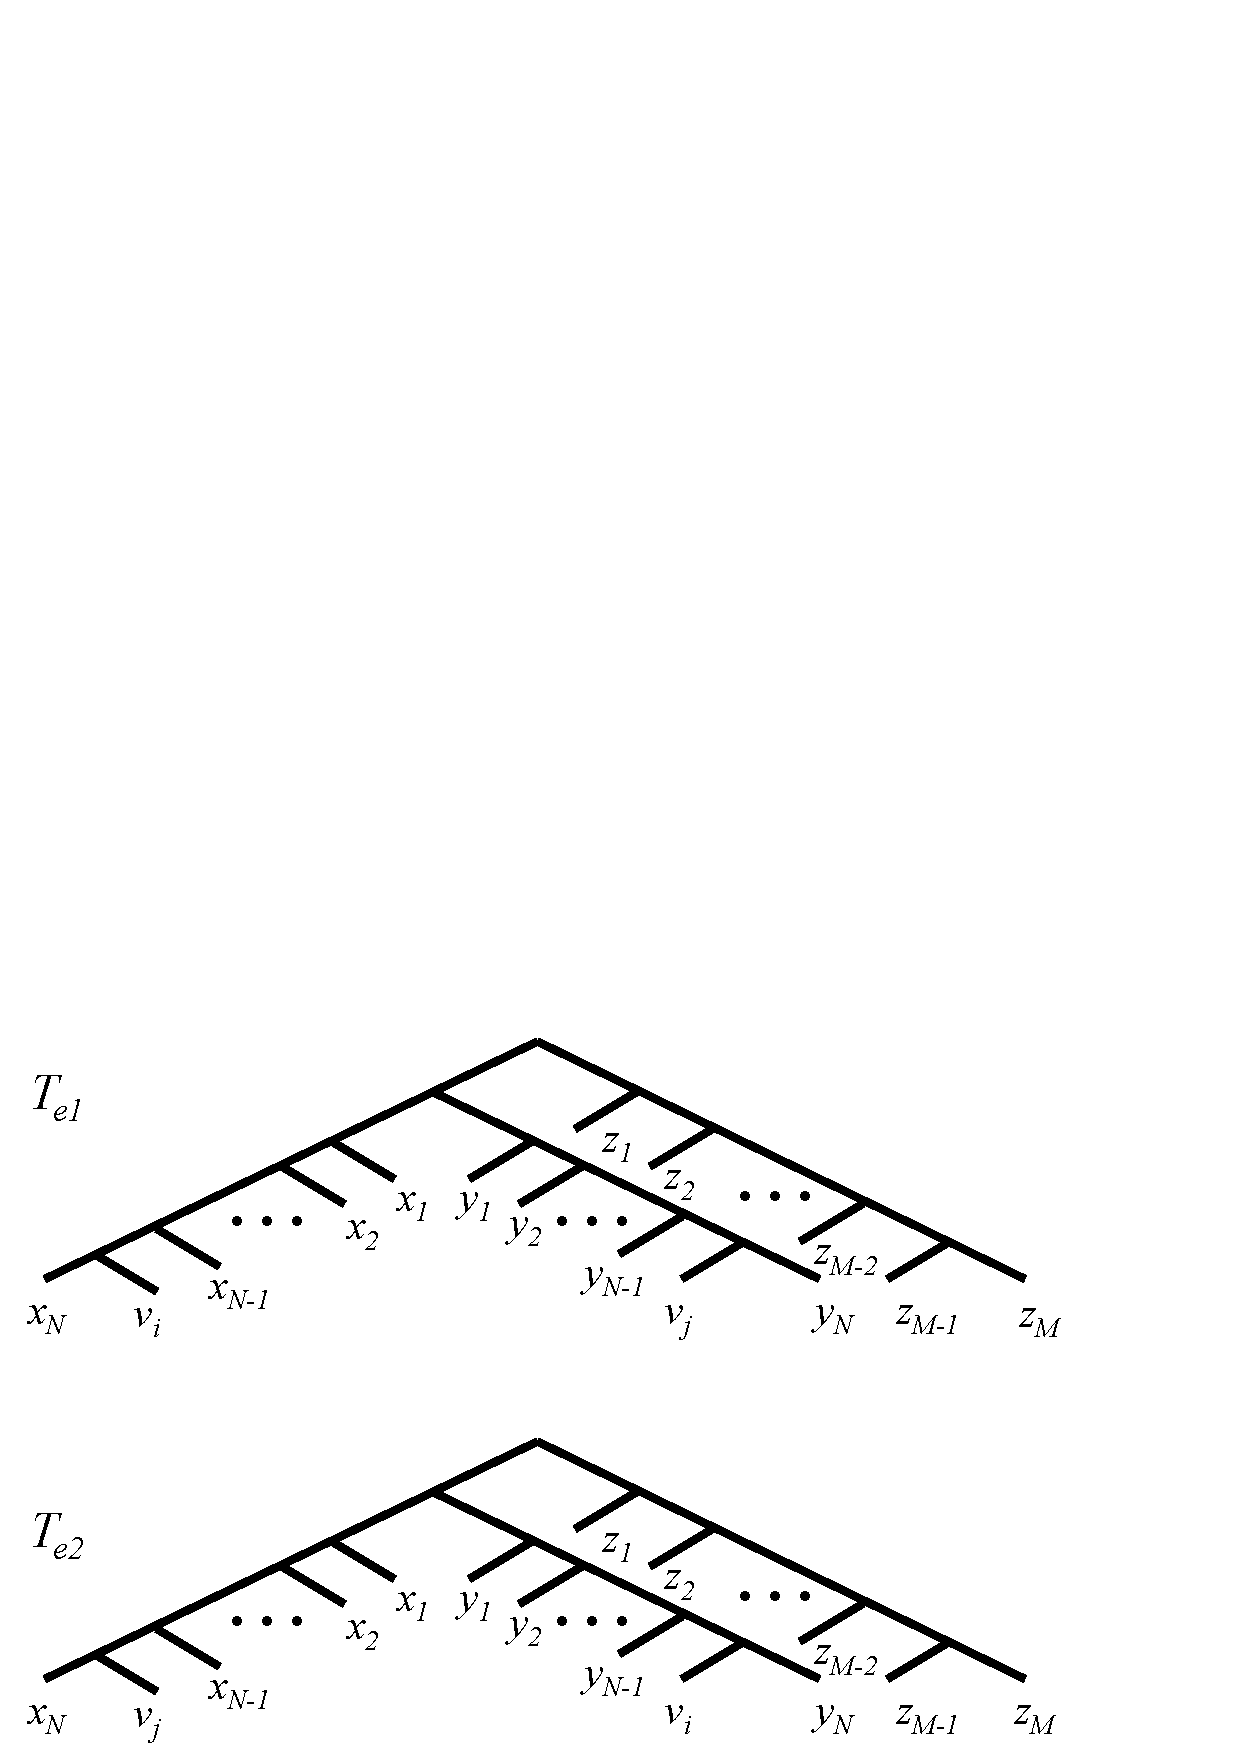
\includegraphics[width=0.9\columnwidth]{Figure3}
\end{center}
\caption{Gene trees defined for each edge $e=(v_i, v_j)$.}
\label{EdgeTrees}
\end{figure}

\section{NP-hardness of the Species Tree Problem}

The parsimony criterion is often used for inference  in biology.
Hence, inferring  a species tree from  a set of gene trees is
usually formulated as the following algorithmic problem.

\noindent {\bf Species Tree Problem}\\
{\sc Input}: A set of gene trees $G_i$, $1\leq i\leq n$.\\
{\sc Solution}: A species tree $S$ that minimizes the total cost
    $\sum_{i} c(G_i, S)$, where $c( , )$ is a reconciliation cost function.

\begin{figure}[t!]
\begin{center}
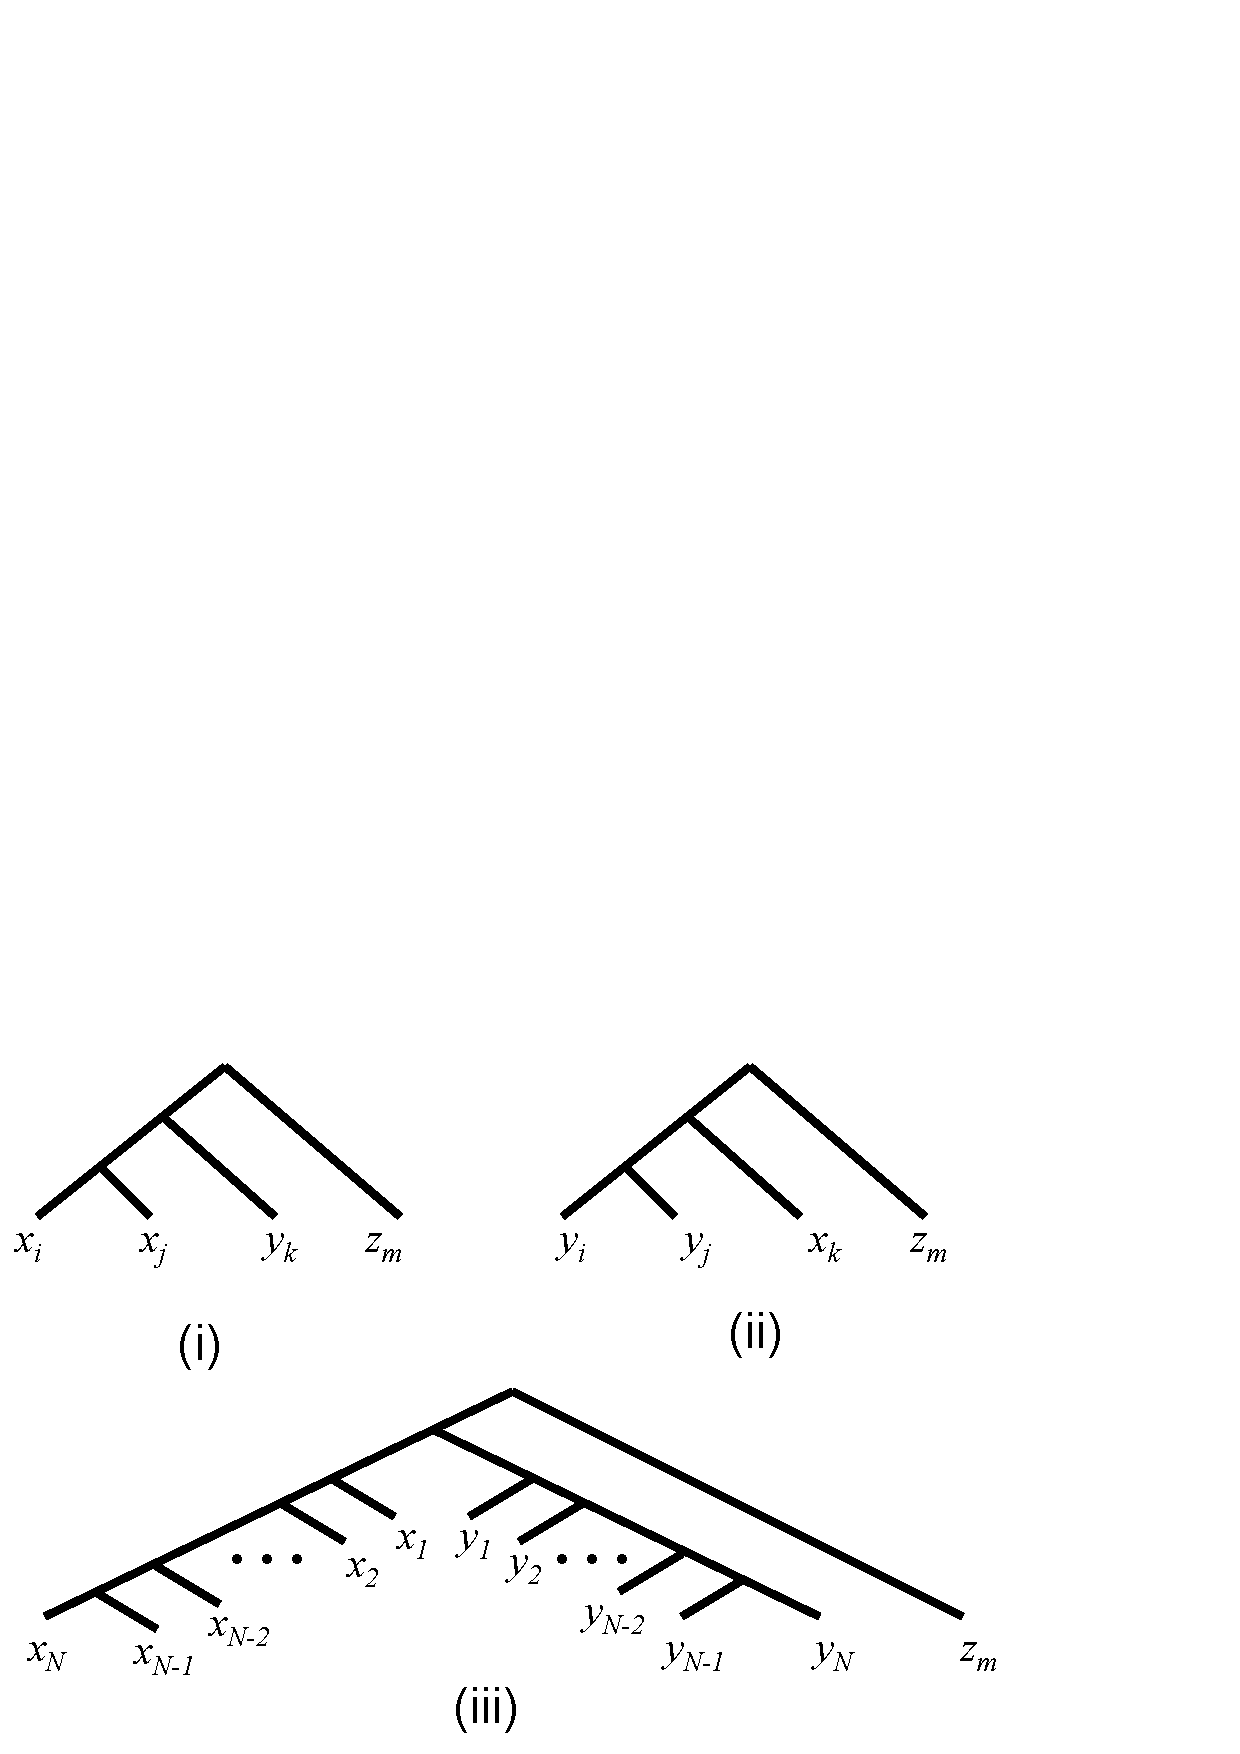
\includegraphics[width=0.9\columnwidth]{Figure4}
\end{center}
\caption{`Structural' gene trees with parameters $i, j, k, m$.}
\label{Gaget_Trees}
\end{figure}

It is proved that the species tree problem is NP-hard for the
duplication and loss costs in \cite{Ma_SIAMComput_01}, which can
also be generalized to the duplication plus loss cost. In this
section, we prove the following theorem.



\begin{theorem}
The species tree problem is NP-hard under the DC cost.
\end{theorem}
{\bf Proof.} Given a gene tree $G$ and a species tree $S$,
the DC cost $c_{dc}(G, S)$ can be
computed in polynomial time since gene duplications and
losses can be  counted in linear time \cite{Zh97}.
Therefore,  the species tree problem is in NP.

 To prove its NP-hardness, we reduce the Maximum Cut problem to the
 decision version of the species tree problem. Given an instance
 graph ${\cal G}=(V, E)$ and
a positive integer $I$,  the Maximum
 Cut problem is to partition the node set $V$ into two disjoint
 subsets $V_1$ and
 $V_2$ such that there are at least $I$  edges from $E$ that have one
 endpoint in $V_1$ and one endpoint in $V_2$.  Assume
 that $V=\{v_1, v_2, \cdots, v_n\}$ and $|E|$ denotes the number of
 edges in $E$, where $n>3$. We construct a
 set $\cal A$ of gene trees to obtain a corresponding instance of the
 species tree problem.



 Choose  $N>n^2$ and $M\geq n^2N(N+1)+ |E|$.
 For each node $v_i$ ($1\leq i\leq n$), we introduce a label with the same
name $v_i$. We
 also introduce $2N+M$ extra labels $x_i, y_i$, $1\leq i\leq N$ and $z_j$, $1\leq j\leq M$.
 For each edge $e=(v_i, v_j) \in E$, we add to $\cal A$ two gene trees $T_{e1}$ and
 $T_{e2}$ as shown in Fig.~\ref{EdgeTrees}.
These two trees are same except that  the leaf labels $v_i$ and  $v_{j}$ are
swapped.



 Let the trees shown in Fig.~\ref{Gaget_Trees} (i)-(iii) be written as
 %$L[x_i, x_j, y_k, z_m]$, $L[y_i, y_j, x_k, z_m]$
 $G_{(i, j, k, m)}$,  $G'_{(i, j, k, m)}$
 and $F[\{x_i\},\{y_i\}, z_m]$, respectively. Besides the `edge' gene trees $T_{e1}$
and $T_{e2}$ ($e\in E)$, the set $\cal A$ of gene trees  also
contains
 \begin{eqnarray*}
   & G_{(i, j, k, m)}, \;1\leq i, j, k \leq N,\;i<j, \; 1\leq m\leq M,\\
   &G'_{(i, j, k, m)}, \;1\leq i, j, k \leq N,\;i<j, \; 1\leq m\leq M,\\
   &G''_{m}=F[\{x_i\},\{y_i\}, z_m],\; 1\leq m\leq M.
 \end{eqnarray*}
These three classes of gene trees are introduced to restrict the
topology of the optimal species tree for the defined instance of the
problem. Hence, we call them `structural' gene trees.
 The NP-completeness of the decision version of the species tree problem
follows from the following two lemmas. Although the proof is long,
the idea is quite simple. The parameter $M$ is set so large that the
structural gene trees will force the species trees with the minimum
DC cost to be three line subtrees joined together as shown in
Fig.~\ref{SpeciesTree},  one of which contains $x_i$s and some
$v_j$s, giving a cut of the graph $\cal G$.



\begin{figure}[t!]
\begin{center}
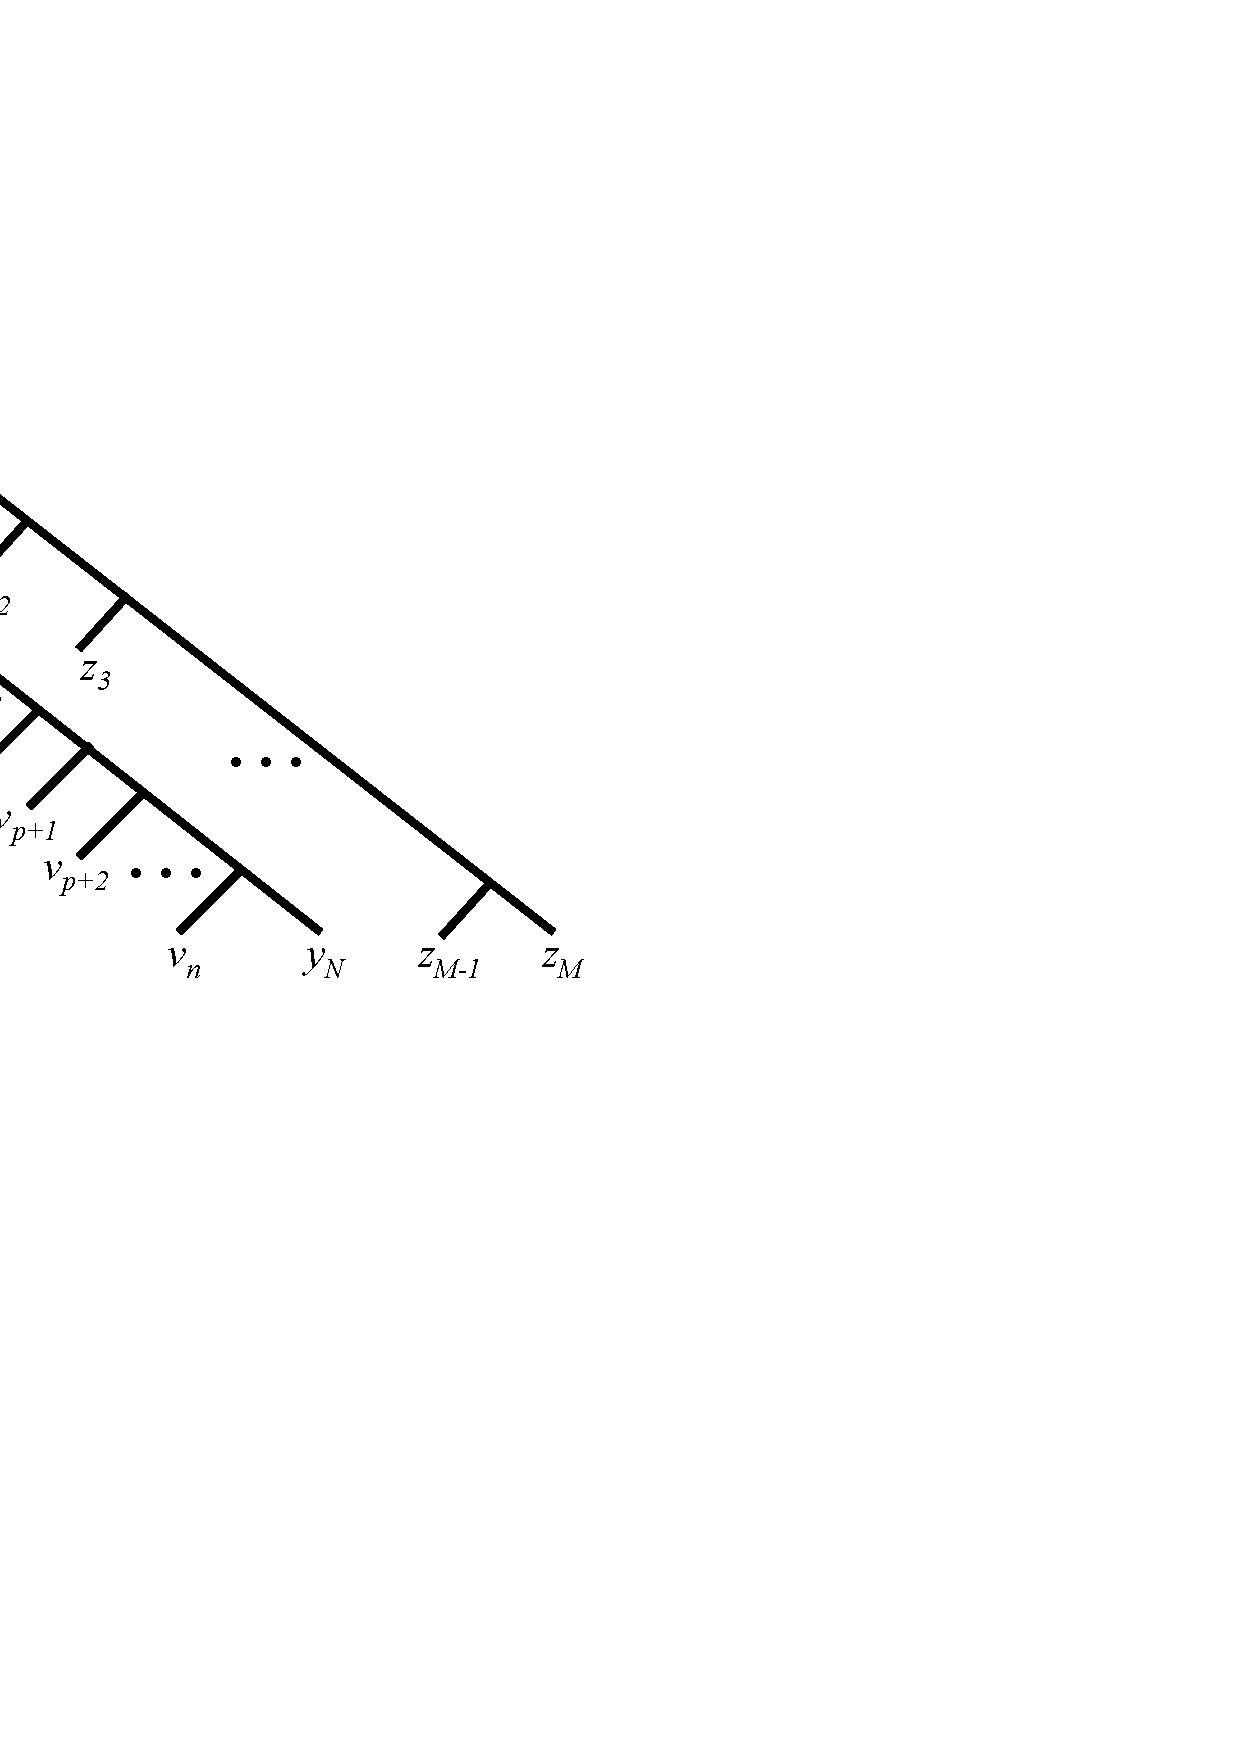
\includegraphics[width=0.9\columnwidth]{Figure5}
\end{center}
\caption{Species tree $S_{\cal G}$ defined from a cut $(V_1, V_2)$
of $\cal G$ in Lemma~\ref{lemma1}.}
 \label{SpeciesTree}
\end{figure}

 \begin{lemma}
\label{lemma1}
   If the graph $\cal G$ has a cut of $d$ edges, there is a
   species tree $S_{\cal G}$ having the DC cost
   $$c_{dc}({\cal A}, S_{\cal G})= N(N+1) |E| + |E| -d.$$
 \end{lemma}
\begin{proof}
  Assume that the node set $V$ of the graph $\cal G$ is divided
 into $V_1=\{v_1,v_2, \cdots, v_p\}$ and $V_2=\{v_{p+1},
 v_{p+2}, \cdots, v_n\}$ such that there are exactly $d$ edges having one
 endpoint in $V_1$ and one endpoint in $V_{2}$.  We define a species
 tree $S_{\cal G}$ as shown in Fig.~\ref{SpeciesTree}.

  First, we observe that
 \begin{eqnarray*}
   & c_{dc}(G_{(i, j, k, m)}, S_{\cal G})=0, &\\
   & c_{dc}(G'_{(i, j, k, m)}, S_{\cal G})=0, &\\
   & c_{dc}(G''_{m}, S_{\cal G})=0,&
 \end{eqnarray*}
for each possible $i, j,k, m$.



 Consider a non-cut edge $e=(v_i, v_j)$ ($i<j$). Since
$L(T_{e1})=L(T_{e2})\subset L(S_{\cal G})$,
$$c_{dc}\left(T_{e1}, S_{\cal G}\right)=c_{dc}\left(T_{e1}, S_{\cal G}|_{L(T_{e1})}\right)$$
 and
$$c_{dc}\left(T_{e2}, S_{\cal G}\right)=c_{dc}\left(T_{e2}, S_{\cal
G}|_{L(T_{e2})}\right).$$

To determine these DC costs, we consider $S_{\cal G}|_{L(T_{e1})}$.
 Without loss of generality, we assume $v_i, v_j \in V_1$ and hence
 $S_{\cal G}|_{L(T_{e1})}$ becomes the one shown in Fig.~\ref{Fig6_lemma41}.
 In the reconciliation of $T_{e1}$ and $S_{\cal G}|_{L(T_{e1})}$,, all extra lineages occur in
the line subtrees with $x$'s and $y$'s; there are no deep
coalescence events in the branch $(p(u), u)$ or on branches on the
paths from the root to $z_M$.


 The left child of the root of
 $T_{e1}$ is mapped to $u$;  $p(x_{N})=p(v_i)$ is mapped to $v$ and
  $p(x_k)$ is mapped to the corresponding $p(x_k)$ for each $1\leq k \leq N-1$;
   $p(y_{1}), p(y_2), \cdots, p(y_{N})$ are all mapped to $u$ since
   $v_j$ belongs to the left subtree  and $y_{N}$  belongs to the
  right subtree of $u$. Therefore,
   there is exactly one
   extra lineage in each of the $N+1$ branches on the path from $u$ to $p(v_j)$.
   In addition, since, for each $1\leq k\leq N$, the branch $(p(y_k), y_k)$
   of $T_{e1}$ is mapped the path from $u$ to $y_k$, there are $N-1$
   extra lineages  on the branch $(u, p(y_1))$ and $N-k$ extra
   lineages on the branch $(p(y_{k-1}), p(y_{k}))$ for $k\geq 2$.
   In total, we have
    \begin{eqnarray*}
       c_{dc}(T_{e1}, S_{\cal G})= \frac{1}{2}N(N-1)+ N + 1\\
    \end{eqnarray*}
    Similarly,
     \begin{eqnarray*}
c_{dc}(T_{e2}, S_{\cal G})= \frac{1}{2}N(N-1)+ N.
    \end{eqnarray*}



  For each cut edge $e=(v_i, v_j)$ ($i<j$) with one endpoint in $V_1$, say
$v_i\in V_1$, and another  in $V_2$, we
have that
    \begin{eqnarray}
       c_{dc}(T_{e1}, S_{\cal G})=0,&
       c_{dc}(T_{e2}, S_{\cal G})= N(N+1).
    \end{eqnarray}
Therefore, we have
  $$c_{dc}({\cal A}, S_{\cal G})= N(N+1)|E|+|E|-d.$$
This finishes the proof of the lemma.
\end{proof}

\begin{figure}[t!]
\begin{center}
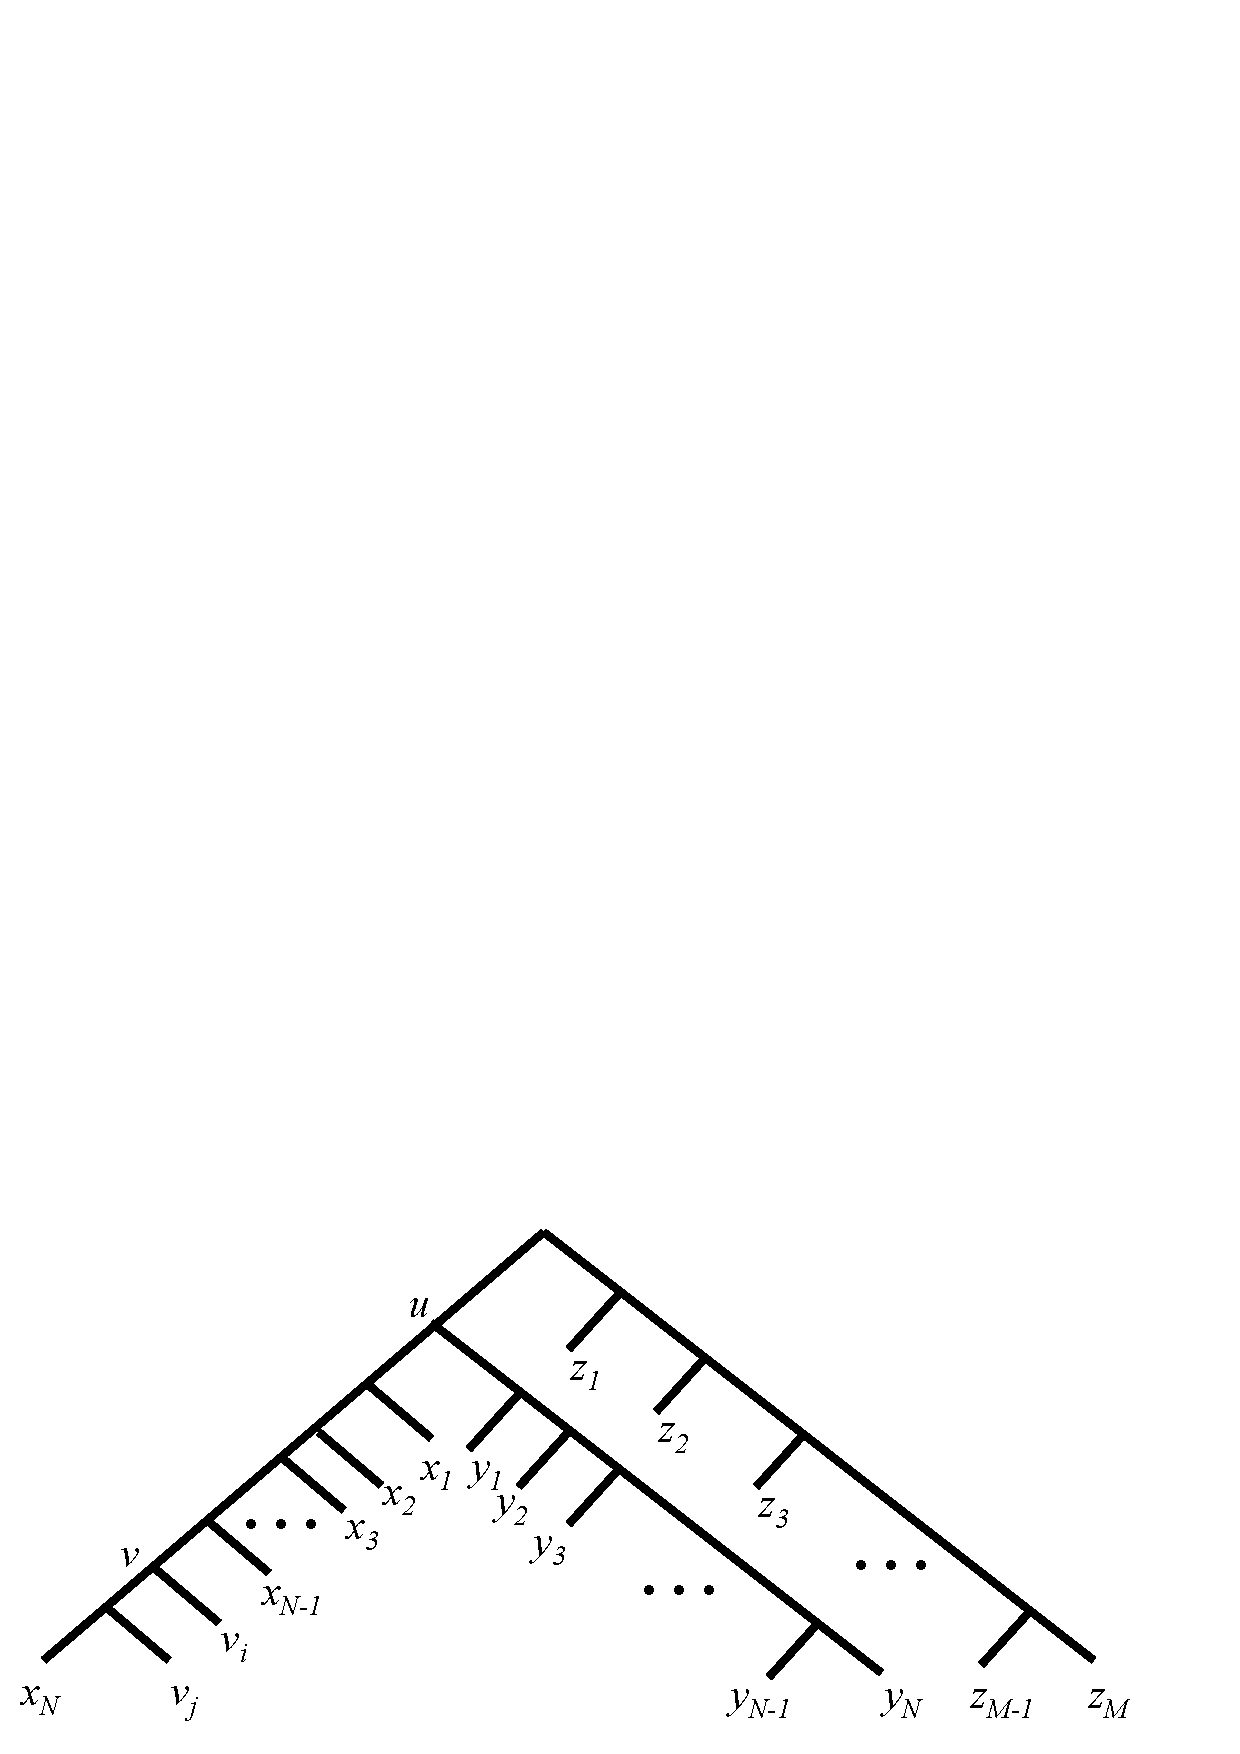
\includegraphics[width=0.9\columnwidth]{Figure6}
\end{center}
\caption{The tree $S_{\cal G}|_{L(T_{e1})}$ defined in
Lemma~\ref{lemma1} when $v_i, v_j\in V_1$ and $i<j$.}
 \label{Fig6_lemma41}
\end{figure}





 \begin{lemma}
\label{lemma2}
    If there is a species tree $S$ having the DC cost
      $c_{dc}({\cal A}, S)=N(N+1)|E| + t$,
         then the graph $\cal G$ has a cut of at least
      $|E|-t$ edges.
 \end{lemma}
\begin{proof}
 %We may assume that $S$ has the smallest DC cost over
If $t> |E|$, the fact is trivial. Hence, without loss of generality,
 we may assume that  $t\leq |E|$.
%
 Here,   we use $\mbox{LT}[a,  \ldots, b,  c]$ to denote the line tree
with leaves labeled by $a$, $b$, $\ldots$, $c$, respectively, as
shown in Fig.~\ref{LineTree} (i). Note that the leaf $a$ is a child
of the root in  $\mbox{LT}[a,  \ldots, b, c]$.
 For a set of trees $T'$, $T''$, $\ldots$,  $T'''$,
we use
 $$\mbox{LT}[T', \ldots, T'',  T''']$$
 to denote the tree
obtained by replacing each leaf by a corresponding subtree in
 $\mbox{LT}[a, \ldots, b,  c]$ as shown in Fig.~\ref{LineTree} (ii).

   Let $B$ be a subset of leaves in the species tree $S$ and  the least common
ancestor of the leaves from $B$  be $r_{B}$ in $S$.   Recall that the
   homomorphic subtree $S|_B$ of $S$ induced by $B$ is the tree
   obtained from $S$ by removing all the nodes and edges that are
   not on a path from $r_B$  to a leaf from $B$ and then
   contracting all the degree-2 node except for the root $r_{B}$.
  For example, for $S_{\cal G}$ defined in Lemma\ref{lemma1},
$S_{\cal G}|_{\{x_1, x_2, y_1\}}=\mbox{LT}[y_1, x_1, x_2]$.


   Set
   \begin{eqnarray}
    &  U=\{x_i, y_i :  1\leq i\leq N\} \cup \{v_1, v_2, \cdots, v_n\}, & \nonumber\\
  %\cup \{ y_i : 1\leq i\leq N\} \cup \{ v_i : 1\leq i\leq N\}; & \nonumber \\
      & Z=\{z_1, z_{2}, \cdots, z_M\}.&
     \end{eqnarray}
   By replacing the children of a two-leaf rooted tree with $S|_{U}$ and
   $S|_{Z}$, we obtain a species tree $S'=\mbox{LT}[S|_{U}, S|_{Z}]$ from S.
 First, $S'$ has the following property.
\vspace{0.5em}

\begin{figure}[t!]
\begin{center}
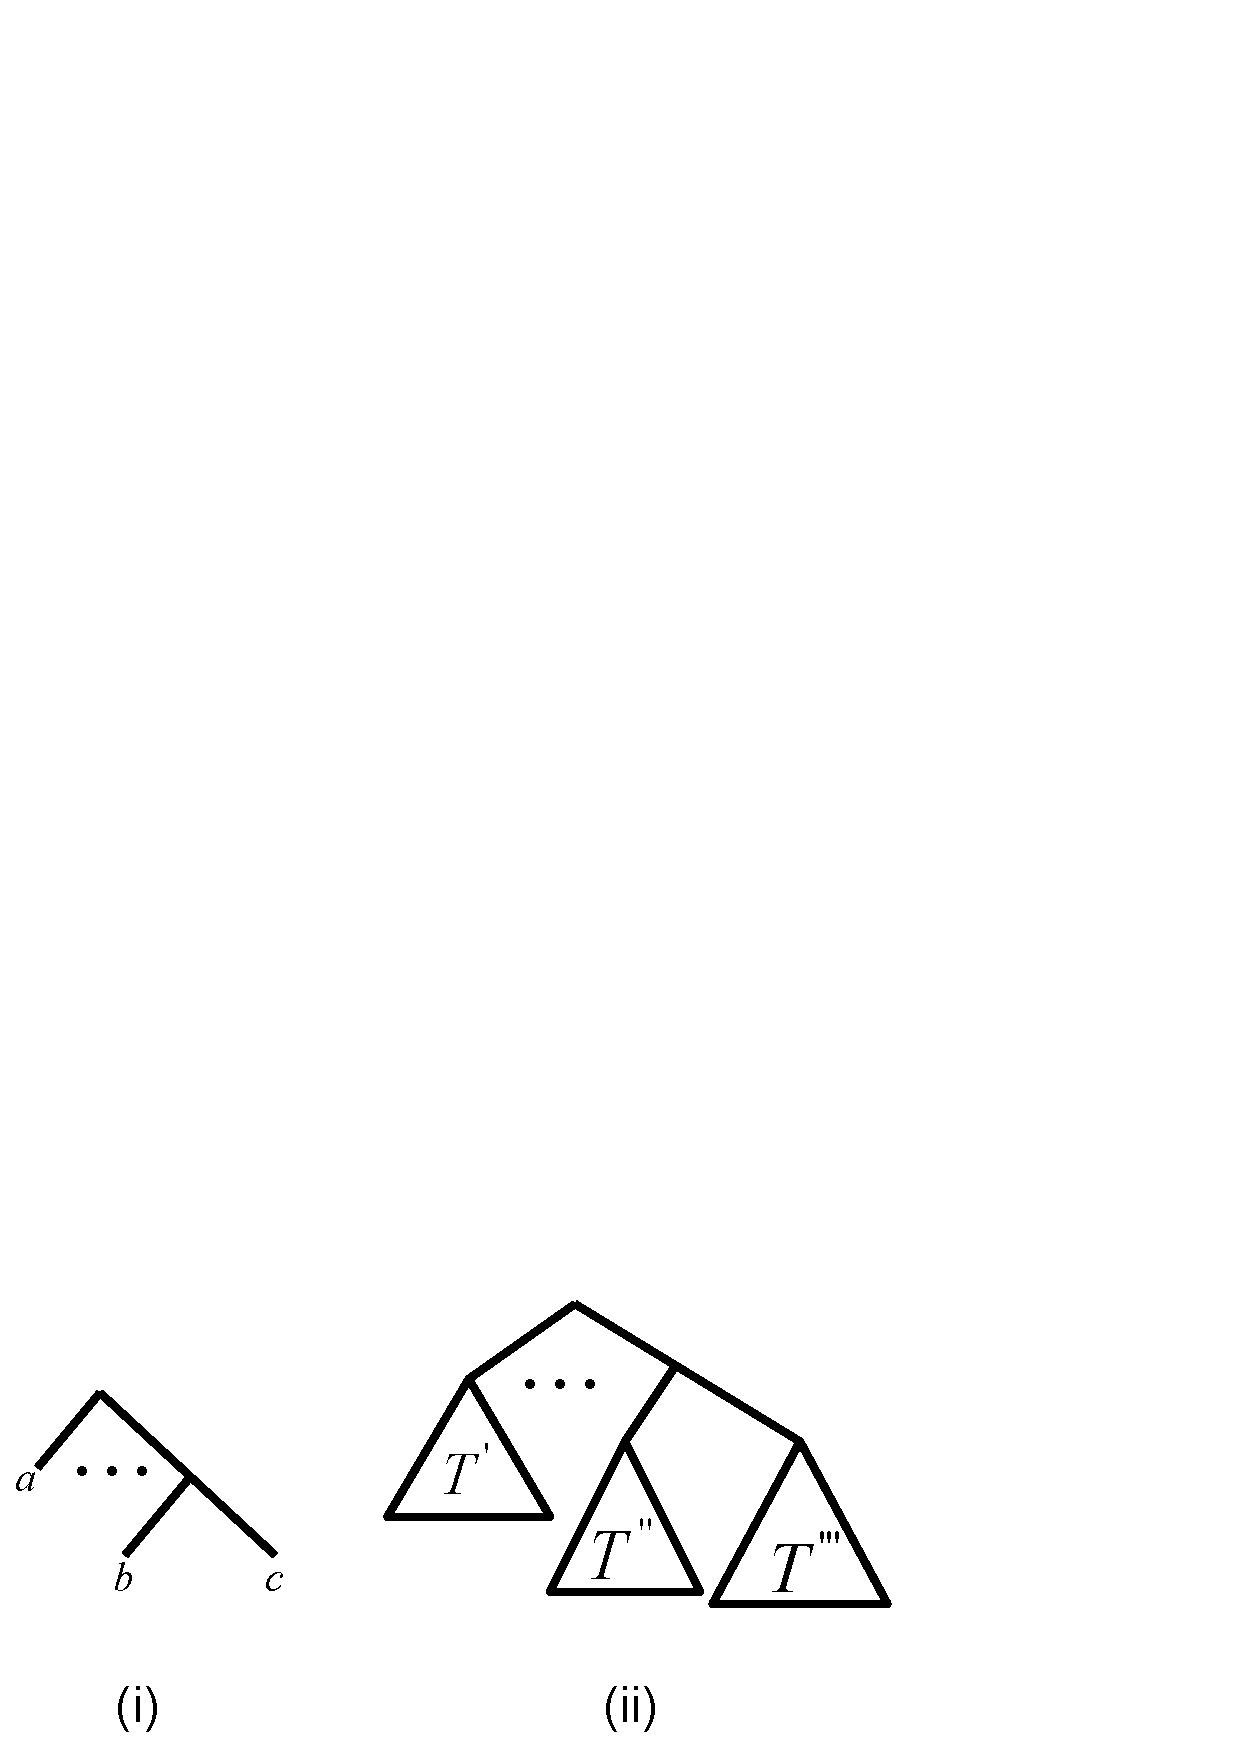
\includegraphics[width=0.7\columnwidth]{Figure7}
\end{center}
\caption{(i) Line tree $\mbox{LT}[a, \ldots, b, c]$. (ii) The
resulting tree $\mbox{LT}[T', \ldots, T'', T''']$ after replacing
each leaf with a tree in a line tree.} \label{LineTree}
\end{figure}

\noindent   {\bf Fact 1}  $c_{dc}({\cal A}, S') \leq c_{dc}({\cal A}, S)=N(N+1)|E| + t$.

\noindent {\bf Proof.} For each gene tree $T=T_{e1}$ or $T_{e2}$, we
use $f$ and $f'$ to denote the lca  mappings from $T$ to $S$ and
$S'$, respectively. Let $r$ be the root of $T$. Assume that $a(r)$
is the left child of $r$,  the least common ancestor of $x_i$s and
$y_i$s,  and $b(r)$  the right child of $r$.
  For each edge $e=(u_1, u_2)$ on a path from $b(r)$ to some $z_i$,
by the definition of $S|_{Z}$,
$$d(f'(u_1), f'(u_2)) \leq d(f(u_1),
f(u_2)),$$ and, furthermore,
 $f(u_1)=f(u_2)$ if and only if
$f'(u_1)=f'(u_2)$.
 For each edge below $a(r)$,
the same property holds. However, the edges incident to the root of
$T$ may not satisfy the property discussed above. It is possible
that $f(r)=f(a(r))$ and/or $f(r)=f(b(r))$. However, $f'(r)=r'$,
$f'(a(r))=a(r')$ and $f'(b(r))=b(r')$, where $r'$ is the root of
$S'$, $a(r')$ and $b(r')$
 the root of $S|_{U}$ and $S|_{Z}$ respectively.
 Since no other lineages fail to coalesce with
$(r, a(r))$  on $(r', a(r'))$ and with $(r, b(r))$ on
 $(r', b(r'))$ respectively, these two edges
does not contribute the deep coalescence cost. Thus,  $c_{dc}(T,
S')\leq c_{dc}(T, S)$.

  Similarly, we also have the following three inequalities
  \begin{eqnarray*}
    c_{dc}\left(G(i, j, k, m), S'\right) &\leq&  c_{dc}\left(G(i, j, k, m), S\right)\\
    c_{dc}\left(G'(i, j, k, m), S'\right) &\leq & c_{dc}\left(G'(i, j, k, m), S\right)\\
c_{dc}\left(G''(m), S'\right) &\leq&  c_{dc}\left(G''(m), S\right)
\end{eqnarray*}
for any $i, j, k, m$.
 Thus, the fact holds. $\Box$
\vspace{0.5em}


 \noindent  {\bf Fact 2.} In  $S|_{U}$,
   all the leaves $x_i$ must be below one child of
 the root and all the leaves $y_i$ must be below the other child of the root.
 In other words, $S|_{U}=\mbox{LT}[T_1, T_2]$, where
 $T_1$ is a tree over $x_i$ and some $v_i$s and $T_2$ is a tree over $y_i$s and
some $v_j$s.

\noindent {\bf Proof.}
Assume that  the fact is false. There are $x_i, x_j$ and $y_k$ such that
 $S|_{\{x_i, x_j, y_k\}}= (S|_{U})|_{\{x_i, x_j, y_k\}}= \mbox{LT}[x_i,
x_j, y_k]$, or there are $y_i, y_j$ and $x_k$ such that $S|_{\{y_i,
y_j, x_k\}}= (S|_{U})|_{\{y_i, y_j, x_k\}}= \mbox{LT}[y_i,
y_j, x_k]$. If the former is true, then, %for any $1\leq m \leq M$,
 $$c_{dc}\left(G_{(i, j, k, m)}, S'\right) \geq 1, \;1\leq m\leq M.$$
This implies that
$$N(N+1)|E|+t\geq  c_{dc}\left({\cal A}, S'\right) \geq \sum^{M}_{m=1}
c_{dc}\left(G_{(i, j, k, m)}, S'\right)  = M,$$
  contradicting to the fact that  $M\geq N(N+1)n^2$.

If the latter is true, for any $1\leq m\leq M$,
 $$c_{dc}\left(G'_{(i, j, k, m)}, S'\right) \geq 1.$$
  Again, we have that
$c_{dc}\left({\cal A}, S'\right) \geq M$, leading to a
contradiction. $\Box$


  Let $X=\{x_1, x_2, \ldots, x_N\}$ and $Y=\{y_1, y_2, \ldots, y_N\}$.
 Then $S'|_{X}=(S|_{U})|_{X}$ and $S'|_{Y}=(S|_{U})|_{Y}$.
\vspace{0.5em}

\noindent {\bf Fact 3.} $S'|_{X}=\mbox{LT}[x_1, x_2, \ldots, x_{N}]$
and
          $S'|_{Y}=\mbox{LT}[y_1, y_2, \ldots, y_{N}]$.

\noindent {\bf Proof.}  Note that
 $G''_{m}|_{X}=\mbox{LT}[x_1, x_2, \ldots, x_{N}]$
and  $G''_{m}|_{Y}=\mbox{LT}[y_1, y_2, \ldots, y_{N}]$ for any
$1\leq m\leq M$. If the claim is false, then,
 $c_{dc}\left(G''_{m}, S'\right) \geq 1$ for any $m$ and hence
$$N(N+1)|E|+t\geq  c_{dc}\left({\cal A}, S'\right) \geq \sum^{M}_{m=1}
c_{dc}\left(G''_{m}, S'\right)  = M,$$ a contradiction as in the
proof of Fact 2. $\Box$
\vspace{0.5em}

Let  the least common ancestor of $x_i$s and $y_i$s be  $w$ in $S'$.
We have shown that $x_i$s are below one child of $w$, say $w_1$, and
$y_i$'s are below the other child of $r$, say $w_2$. Recall that
$S'|_{X}$ and $S'_{Y}$ are two line trees.
\vspace{0.5em}

\noindent {\bf Fact 4.}  For each edge $e=(v_i, v_j)$ ($i<j$) such that
          $v_i$ and $v_j$ are in the same subtree as $x_i$s or as $y_i$s,
         then
 $$c_{dc}\left(T_{e1}, S'\right)+ c_{dc}\left(T_{e2}, S'\right)\geq N(N+1)+1.$$

\noindent  {\bf Proof.} Without loss of generality, we may assume that
         $v_i$ and $v_j$ are  below $w_1$ in the same subtree as $x_i$s.
We consider the
 following two cases.

  If
  \begin{eqnarray*}
  & & S|_{X\cup \{v_i, v_j\}}\\
  & =& \mbox{LT}[x_1, x_2, \cdots, x_k, v_i, x_{k+1},
    \cdots, x_{m}, v_j, v_{m+1}, \cdots, x_{N}]
    \end{eqnarray*}
     for some
 $0\leq k\leq m\leq N$,  we have that
     $$ c_{dc}\left(T_{e1}, S'\right) = \frac{1}{2}N(N-1)+N+1 + \frac{1}{2}(N-k)(N-k-1)$$
and
     $$ c_{dc}\left(T_{e2}, S'\right) = \frac{1}{2}N(N-1)+k+1 + \frac{1}{2}(N-m)(N-m-1).$$
Hence,
{\small
\begin{eqnarray*}
  & & c_{dc}\left(T_{e1}, S'\right)+ c_{dc}\left(T_{e2}, S'\right)\\
  & \geq  & N(N-1) + N+1 + \frac{1}{2} [(N-k)(N-k-1)+ 2k+2]\\
  &  \geq &  N(N+1)+1
\end{eqnarray*}
}
 as the minimum value of $(N-k)(N-k-1)+ 2k+2$ is $N$ (reaching at
$k=N-2, N-1$).


    If
    \begin{eqnarray*}
    && S|_{X\cup \{v_i, v_j\}}\\
    &=&\mbox{LT}[x_1, x_2, \cdots, x_k,
 \mbox{LT}[v_i, v_j],  x_{k+1},
    \cdots, x_{N-1},  x_{N}]
    \end{eqnarray*}
    for some $0\leq k\leq N$,
  we have that
  {\small
     $$ c_{dc}\left(T_{e1}, S'\right)
  = \frac{1}{2}N(N-1)+k+2 + \frac{1}{2}(N-k)(N-k-1)$$
  }
  and
  {\small
   $$c_{dc}\left(T_{e2}, S'\right)
  = \frac{1}{2}N(N-1)+k+2 + \frac{1}{2}(N-k)(N-k-1).$$
  }
Therefore,
\begin{eqnarray*}
 & & c_{dc}\left(T_{e1}, S'\right)+ c_{dc}\left(T_{e2}, S'\right)\\
 & \geq & N(N-1) + 2k+4 + (N-k)(N-k-1)\\
 &  \geq &  N(N+1)+2
\end{eqnarray*}
as the minimum value of $2k+(N-k)(N-k-1)$ is  2N-2 (reaching at $k=N-1, N-2$).
The fact is proved. $\Box$
\vspace{0.5em}

\noindent {\bf Fact 5.}  For each edge $e=(v_i, v_j)$ such that
$v_i$ is  below $w_1$ in the same subtree as $x_i$ and $v_j$ is
below $w_2$  in the subtree as $y_i$s. Then,
 $$c_{dc}\left(T_{e1}, S'\right)+ c_{dc}\left(T_{e2}, S'\right)\geq N(N+1).$$

\noindent {\bf Proof.} Let
$$S|_{X\cup \{v_i\}}=\mbox{LT}[x_1, x_2,\cdots,x_{k}, v_i, x_{k+1},
\cdots, x_{N-1}, x_{N}]$$ and
$$S|_{Y\cup \{v_j\}}=\mbox{LT}[y_1, y_2,\cdots,y_{m}, v_j, y_{m+1},
\cdots, y_{N-1}, y_{N}].$$

We have that all the internal nodes in $T_{e2}$ are mapped onto the
least common ancestor $w$  of $x_i$s and $y_j$s and thus
  $$ c_{dc}\left(T_{e2}, S'\right)= N(N+1).$$
Since $c_{dc}\left(T_{e1}, S'\right)\geq 0$, the fact is proved.
$\Box$
\vspace{0.5em}


 Let $V_1$ denote the subset of leaves $v_i$ below $w_1$ in the same subtree as
$x_i$s and $V_2$ the subset of leaves $v_j$ below $w_2$
 in the same subtree as $y_i$s.
Then $(V_1, V_2)$ is a cut of the graph $\cal G$. Assume there are $p$ cut edges.
Since there are $|E|-p$ non-cut edges,
\begin{eqnarray*}
  & & N(N+1)|E|+t\\
  &= & c_{dc}({\cal A}, S')\\
  & \geq & (|E|-p)N(N+1) + pN(N+1) + (|E|-p)\\
  & = & N(N+1)|E| + |E|-p,
  \end{eqnarray*}
which implies that $p\geq |E|-t$. This  finishes the proof of
Lemma~\ref{lemma2}.
\end{proof}

\section{Conclusion}

We conclude this paper by posing three related research problems. In
this paper, we have proved that species tree inference by minimizing
deep coalescences is NP-hard. This justifies the effort from
different groups in seeking efficient heuristic methods for the
inference problem \cite{Maddison_SysBiol_06, Tran_PlosCB_09}. We
have also discussed the relationship of the deep coalescence cost
and the gene duplication cost. There are two research problems arising
 from this study. Does the species tree inference problem remain NP-hard if
every gene tree has the same set of taxon labels? Is there any
polynomial-time algorithm with constant approximation ratio for the
species tree problem in the deep coalescence model? Note that the
heuristic method developed by Than and Nakhleh in
\cite{Tran_PlosCB_09} seems to be effective.

The parametric complexity of the species tree inference by
minimizing gene  duplications has been studied in the past several
years. Is it possible to develop efficient algorithms for parametric
species tree inference under the deep coalescence model?






\section*{Acknowledgements}

The author would like to thank four anonymous reviewers for their
useful commentary. LX Zhang was financially supported
by AcRF R146-000-109-112. A
preliminary version of this work was presented in the poster session
of the RECOMB'2000.


\begin{thebibliography}{99}

\bibitem{Bansal_TCBB_08}
M.S. Bansal and O. Eulenstein,
 ``The multiple gene duplication problem revisited",
{\it Bioinformatics}, vol. 24, pp. 132-138, 2008.

\bibitem{Chauve_JCB_08}
C. Chauve, J.P. Doyon, and N. El-Mabrouk,  ``Gene family evolution
by duplication, speciation, and loss",  {\it J. Comput. Biol.}, vol.
15, pp. 1043-1062, 2008.

\bibitem{Chen_JCB_00}
K. Chen, D. Durand, and M. Farach-Colton,  ``Notung: A program for
dating gene duplications and optimizing gene family trees",
 {\it  J. Comput.  Biol.}, vol. 7, pp. 429-447, 2000.

\bibitem{Degan_Evol_05}
J.H. Degnan and L.A. Salter, ``Gene tree distribution under the
coalescence process", {\it Evolution}, vol. 59, pp. 24-37, 2005.

\bibitem{Doyle_SysBot_92}
J.J. Doyle,  ``Gene trees and species trees: molecular
 systematics as one-character taxonomy",  {\it Syst. Bot.}, vol. 17,
 pp. 144-163, 1992.

\bibitem{Durand_JCB_06}
D. Durand, B.V. Halldorsson, and B. Vernot, ``A hybrid
micro-macroevolutionary approach to gene tree reconstruction",
 {\it  J. Comput. Biol.}, vol. 13, pp. 320-335, 2006.

\bibitem{Edwards_Evolution_00}
S.V. Edwards and P. Beerli, ``Perspective: gene divergence,
population divergence, and the variance in coalescence time in
phylogeography studies",  {\it Evolution}, vol. 54, pp.  1839-1854,
2000.

\bibitem{Eulenstein_JCB_98}
O. Eulenstein, B. Mirkin, and M.  Vingron, ``Duplication-based
measures of difference between gene and species trees",  {\it J.
Comput. Biol.}, vol. 5, pp. 135-148, 1998.



\bibitem{Fitch_SysZool_70}
W. Fitch,  ``Distinguishing homologous from analogous proteins",
{\it Syst. Zool.}, vol. 19, pp. 99-113, 1970.

\bibitem{Garey_Book_79}
M. Garey and D. Johnson,  {\it Computers and Intractability: A Guide
to the Theory of NP-completeness},
 W.~H.~Freeman, New York, 1979.

\bibitem{Goodman_SysZool_79}
M. Goodman, J. Czelusniak,  G.W. Moore, A.E. Romero-Herrera, and G.
Matsuda,  ``Fitting the gene lineage into its species lineage, a
parsimony strategy illustrated by cladograms constructed from globin
sequences", {\it Syst. Zool.}, vol. 28, pp. 132-163, 1979.

\bibitem{Guigo_MPE_96}
R.  Guig\'{o}, I. Muchnik, and T. Smith, ``Reconstruction of ancient
molecular phylogeny", {\it Mol. Phylogenet. Evol.}, vol. 6, pp.
189-213, 1996.

\bibitem{Hallett_Recomb00}
M.T. Hallett and J. Lagergren,  ``New algorithms for the
duplication-loss model",  In {\it Proceedings of RECOMB'2000}, pp.
138-146, 2000.

\bibitem{Hey_Genetics_04}
J. Hey and R. Nielsen,
 ``Multilocus methods for estimating population
sizes, migration rates and divergence time, with applications to the
divergence of {\it Drosophila pseudoobscura} and {\it D.
persimilis}", {\it Genetics}, vol. 167, pp. 747-760, 2004.

\bibitem{Hadas_JCB_09}
R. Libeskind-Hadas and M.A. Charleston,  ``On the computational
complexity of the reticulate cophylogeny reconstruction problem",
{\it J. Comput. Biol.}, vol. 16, pp. 105-117, 2009.


\bibitem{Liu_MPE_09}
L. Liu, L.L. Yu, L. Kubatko, D.K. Pearl, S.V. Edwards, ``Coalescent
methods for estimating phylogenetic trees",  {\it Mol. Phylogenet.
Evol.}, vol. 53, pp. 320-328, 2009.

\bibitem{Luo_TCBB_10}
C.W. Luo, M.C. Chen, Y.C. Chen, W.L. Yang, H.F. Liu, and K.-M. Chao,
``Linear-time algorithms for the multiple gene duplication
problems",  {\it IEEE Trans. Comput Biol. and Bioinform.} (in
press), 2010.

\bibitem{Ma_SIAMComput_01}
B. Ma, M. Li and L.X. Zhang, ``From gene trees to species trees",
{\it SIAM J. Comput.}, vol. 30, pp. 729-752, 2001.

\bibitem{Maddison_SysBiol_97}
W.P. Maddison,
 ``Gene trees in species trees", {\it Syst. Biol.}, vol. 46, pp. 523-536,
 1997.

\bibitem{Maddison_SysBiol_06}
W.P. Maddison and L. Knowles, ``Inferring phylogeny despite
incomplete lineage sorting",  {\it Syst. Biol.}, vol. 55, pp.
21-30, 2006.

\bibitem{Mirkin_JCB_95}
 B. Mirkin, I. Muchnik and T. Smith,
 ``A biologically meaningful model for comparing molecular phylogenies",
 {\it J. Comput. Biol.}, vol. 2, pp. 493-507, 1995.

\bibitem{Miyamoto_SysBiol_95}
M.M. Miyamoto and W.T. Fitch, ``Testing species phylogenies and
phylogenetic methods with congruence",  {\it Syst. Biol.}, vol. 44,
pp. 64-76, 1995.

\bibitem{Nei_Book_87}
M. Nei,
   {\it Molecular Evolutionary Genetics}, Columbia University Press,
    New York, 1987.

\bibitem{Page_SysBiol_94}
R. Page,  ``Maps between trees and cladistic analysis of historical
associations among genes, organisms, and areas", {\it Syst. Bio.},
vol. 43, pp. 58-77, 1994.
%
\bibitem{Page_MPE_97}
R. Page and   M. Charleston,  ``From gene to organismal phylogeny:
reconciled trees and the gene tree/species tree problem", {\it Mol.
Phylogenet. Evol.}, vol. 7, pp. 231-240, 1997.
%
\bibitem{PN88}
P. Pamilo and M. Nei,  ``Relationship between gene trees and species
trees", {\it Mol. Biol. Evol.}, vol. 5, pp. 568-583, 1988.

\bibitem{Ronquist_ZoolScr_97}
F. Ronquist,  ``Phylogenetic approaches in coevolution and
biogeography",  {\it Zool. Scripta}, vol.  26, pp.  313-322, 1997.

\bibitem{Rosenberg_TheorPopBiol_2002}
N.A. Rosenberg, ``The probability of topological concordance of gene
trees and species trees", {\it Theor. Popul. Biol.}, vol.  61, pp.
225-247, 2002.


\bibitem{Roth_JExpZool_07}
C. Roth, A. Rastogi, L. Arvestad, K. Dittmar, S. Light, D. Ekman, A.
David, and D.A. Liberles,
 ``Evolution after gene duplication: models, mechanisms,
sequences, systems, and organisms",  {\it J Exp. Zool. Part B}, vol.
308, pp.  58-73, 2007.

%\bibitem{Fellows_JA_03}
%U. Stege,   ``Gene Trees and Species Trees: The Gene-Duplication
%Problem in Fixed-Parameter Tractable",  In {\it Proceedings of
%WADS}, pp. 288-293, 1999.

\bibitem{T89}
 N. Takahata,
 ``Gene genealogy in three related population:
 Consistency probability between gene and population trees",
{\it Genetics}, vol. 122, pp. 957-966, 1989.
%
\bibitem{Tran_PlosCB_09}
C. Than and L. Nakhlen,  ``Species tree inference by minimizing deep
coalescences",  {\it PLoS Comput. Biol.}, vol. 5,
e1000501.doi:10.1371/journal.pcbi.1000501, 2009.

%
\bibitem{Wu91} C.-I. Wu,
``Inference of species phylogeny in relation to segregation of
ancient polymorphisms",  {\it Genetics}, vol. 127, pp. 429-435,
1991.

\bibitem{Zh97}
L.X. Zhang,
 ``On a Mirkin-Muchnik-Smith conjecture for comparing
molecular phylogenies",  {\it J. Comput. Biol.},  vol. 4, pp.
177-188, 1997.

\end{thebibliography}

\newpage


\section*{Figure and table captions}

{\bf Figure 1}: (i) A gene tree. (ii) A species tree. (iii) The reconciliation of  the gene tree in (i) and
 the species tree in (ii) has deep coalescence cost 3.
\vspace{1em}

\noindent
{\bf Figure 2}:  (i) A gene tree. (ii) A species tree. In the lca  reconciliation $M$
  of the gene tree with the species tree,   $a$ is mapped to the left highlighted node,
$b, c, d, e, f$ and $r$ to the root, and $g$ to the right highlighted node.
The nodes $b, c, d, e, f, r$ form a subtree of the gene tree.
\vspace{1em}

\noindent 
{\bf Figure 3}:  Gene trees defined for each edge $e=(v_i, v_j)$.
\vspace{1em}

\noindent 
{\bf Figure 4}: `Structural' gene trees with parameters $i, j, k, m$.
\vspace{1em}



\noindent 
{\bf Figure 5}: Species tree $S_{\cal G}$ defined from a cut $(V_1, V_2)$ of $\cal G$ in Lemma~\ref{lemma1}.
\vspace{1em}

\noindent 
{\bf Figure 6}: The tree $S_{\cal G}|_{L(T_{e1})}$ defined in Lemma~\ref{lemma1} when $v_i, v_j\in V_1$ and $i<j$.
\vspace{1em}

\noindent 
{\bf Figure 7}: (i) Line tree $\mbox{LT}[a, \ldots, b, c]$. (ii) The resulting tree $\mbox{LT}[T', \ldots, T'', T''']$
 after replacing each leaf with a tree in a line tree.
\end{document}
